\documentclass{szzclass}
\usepackage[czech]{babel}

\subject{DBS}
\code{BI-SPOL-10}
\topic{Transakce a jejich vlastnosti - ACID.}

\begin{document}

\tableofcontents
\newpage

\section{Požadavky na konzistenci databáze}

V rámci DBMS (Database Management Service) je potřeba myslet na konzistenci dat a jejich ochranu. Je potřeba
myslet na to, že žádná akce by neměla ohrozit integritu celého systému.

\begin{itemize}
\item Dva základní požadavky na DBMS:
  \begin{itemize}
  \item chránit data – ve smyslu odolnosti vůči různým haváriím serveru
  \item poskytnout korektní, rychlý a asynchronní pčístup vetšímu množství současně pracujících uživatelů.
  \end{itemize}
\item Řešení
  \begin{itemize}
  \item komponenta řízení soubežného (paralelního) zpracování
  \item \item   (concurreny control)
  \item komponenta zotavení z chyb (recovery)
  \end{itemize}
\end{itemize}

\section{Transakce}

Vhodná programová jednotka a vhodné mechanismy, které zabezpečí, že po skončení akce (korektním i nekorektním) zůstane databáze konzistentní (platí všechna IO definovaná ve schématu).

\begin{itemize}
\item COMMIT - potvrzení
\item ROLLBACK - zrušení
\end{itemize}

Stavový diagram transakce

\begin{itemize}
\item aktivní (Active) - od začátku (probíhají DML příkazy)
\item částečně potvrzený (Partially Commited) - po provedení poslední operace transakce
\item potvrzený (Commited) - po úspešném zakončení, tj. po potvrzení operace COMMIT
\item chybný (Failed) - v normálním průběhu transakce nelze pokračovat
\item zrušený (ABorted) - po skončení operace ROLLBACK, tj. uvedení databáze do stavu před započetím transakce
\end{itemize}

\begin{figure}[h!]
  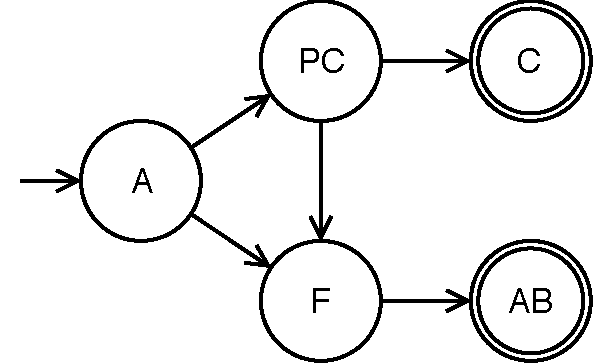
\includegraphics[width=0.5\textwidth]{topics/bi-spol-10/images/state}
  \caption{Stavový diagram transakce}
\end{figure}

\section{ACID vlastnosti transakce}
\begin{itemize}
\item atomicita (Atomicity) - transakce musí buď proběhnout celá nebo vůbec
\item konzistence (Consistency) - transformuje databázi z konzistentního stavu do jiného konzistentního stavu
\item nezávislost (Independence) - dílčí efekty jedné transakce nejsou viditelné jiným transakcím
\item trvanlivost (Durability) - efekty úspěšné transakce jsou trvale uloženy
\end{itemize}

\textbf{Žurnál} obsahuje sekvenci změnových vektorů <XID, pageID, offset, length, old data, new data>
Žurnál a přidružená infrastruktura umožňuje implementaci Atomicity a Durability u transakčního zpracování.
Informace z transakčního žurnálu se používají pouze pro obnovu databáze po chybě.

\section{Rozvrhy}
Stanovení pořadí provádění dílčích akcí více transakcí v čase nazveme \textbf{rozvrhem}. Rozvrh je korektní, když je v nějakém smyslu ekvivalentní kterémukoliv sériovému rozvrhu.

Rozvrh je uspořádatelný (koretní) pokud nemá precendenční graf kružnici.
Rozvrhy jsou ekvivalentní mají-li stejný precendenční graf.

Precendenční graf rozvrhu:
\begin{itemize}
\item uzly = jednotlivé transakce rozvrhu
\item hrany (orientované)
  \begin{itemize}
  \item jedna transakce READ(A) před tím než druhá transakce WRITE(A)
  \item jedna transakce WRITE(A) před tím než druhá transakce READ(A)
  \item posledni WRITE(A) v jende je pred poslednim WRITE(A) v druhe.
  \end{itemize}
\end{itemize}

Paralelní zpracovaní transakcí:
\begin{itemize}
\item Testování uspořádatelnosti
\item Uzamykani (LOCK TABLE)
\end{itemize}

Dvoufázová transakce:
\begin{itemize}
\item 1. fáze - uzamyká se, nic neodemyká
\item 2. fáze - od prvního odemknutí, do konce se už nic nezamyká
\end{itemize}

Dobře formované transakce:
\begin{itemize}
\item transakce zamyká objekt, chce-li k němu přistupovat
\item transakce nezamyká objekt, který již zamkla
\item transakce neodmyká objekt, který nezamkla
\item na konci transakce nezůstane žádný objekt zamčený
\end{itemize}

Jestliže všechny transakce v dané množině transakcí T jsou:

\begin{itemize}
\item dobře formované
\item dvoufázové $\Rightarrow$ pak každý jejich legální rozvrh je uspořádatelný.
\end{itemize}

\end{document}
